\advance\baselineskip by.1pt

\spis{O~przedwiecznej inflacji}
{Mateusz Kulejewski}


\wtyt{\hspace*{-5.5cm}O~przedwiecznej inflacji
\hfill
\waut{Mateusz KULEJEWSKI}}

\rightline{\scriptsize Doktorant na Wydziale Fizyki Uniwersytetu Warszawskiego}
\vspace*{\parskip}
\begin{dwieszpalty}
Komuż z~nas nie zdarzyło się w~godzinie zadumy zapatrzeć w~rozgwieżdżone nocne niebo i~zanurzyć  w~rozmyślaniach nad naszym miejscem w~wielkim Wszechświecie? Jego bogactwo od wieków było natchnieniem dla poetów i~filozofów. Nie bez powodu starożytni Grecy ujrzeli na niebie zmagania swoich bogów, a~w~doskonałej harmonii niebieskich sfer odnaleźli dowód na fundamentalny ład otaczającego ich kosmosu.

Co jednak możemy dostrzec na niebie? Zza wielobarwnego teatru mgławic, gwiazd skupiających się w~galaktyki i~umierających, by pozostawić białe karły, gwiazdy neutronowe i~czarne dziury, czy galaktyk gromadzących się w~gromady galaktyk -- dobiega do nas sygnał szczególny, echo Wszechświata z~czasów, gdy był jeszcze młody. Jest to mikrofalowe promieniowanie tła (z~angielskiego \textit{cosmic microwave background}, CMB), sygnał wyemitowany, gdy Wszechświat miał około trzystu osiemdziesięciu tysięcy lat i~wypełniająca go plazma zrzedniała i~schłodziła się na tyle, by pozwolić światłu spokojnie się rozprzestrzeniać -- co dzieje się do dziś, gdy za pomocą radioteleskopów badamy jego rozkład na niebie.

\marg{
O~CMB pisał Krzysztof Turzyński w~\href{https://www.deltami.edu.pl/2023/12/aktualnosci-pol-wieku-oswajania-wszechswiata/}{$\Delta^{12}\sb{23}$}.
}CMB to dobiegające zewsząd tło o~prawie jednorodnej temperaturze około 2,73 kelwinów -- co odpowiada maksimum długości fali w~promieniowaniu mikrofalowym, stąd jego nazwa. Odkryli je w~1964~roku Penzias i~Wilson, gdy pomimo wielu prób, włącznie z~usunięciem gniazda gołębi %oraz ich innych
z~czaszy radioteleskopu, nie mogli pozbyć się dobiegającego zewsząd szumu. Po 14 latach ich odkrycie zostało uhonorowane Nagrodą Nobla, a~kilkadziesiąt lat później kolejne sondy kosmiczne -- zazwyczaj o~wdzięcznej, skrótowej nazwie, jak COBE czy WMAP lub najnowszy Planck -- mierzą je z~coraz większą dokładnością, by zbadać strukturę wczesnego Wszechświata.

Najbardziej uderzającą własnością CMB jest jego prawie dokładna jednorodność -- w~którą stronę nie spojrzymy, Wszechświat wypełnia niemal identyczny, termiczny szum. Dla fizyków budujących modele kosmologiczne na bazie ogólnej teorii względności jest to obserwacja pożądana. Współczesne modele kosmologiczne opisują tzw. czasoprzestrzeń Friedmanna--Lemaître'a--Robertsona--Walkera (której wieloczłonowa nazwa jest związana z~jej wielokrotnymi, niezależnymi odkryciami).
\marg{O~modelach FLRW i~przyjmowanych w~nich założeniach pisał Szymon Charzyński w~\href{https://deltami.edu.pl/2023/02/modele-wszechswiata-dla-poczatkujacych-czesc-2-upraszczamy-ile-sie-da/}{$\Delta^2\sb{23}$}.}
Podstawą, od której zaczyna się budowę tych modeli, jest przyjęcie założenia zwanego zasadą kopernikańską:  Wszechświat jest jednorodny i~izotropowy, czyli dokładnie taki sam, niezależnie od tego, w~którym jego miejscu się znajdujemy i~w~którą stronę patrzymy. Oczywiście nie jest to założenie spełnione na Ziemi -- na szczęście znacząco się różnimy od naszego otoczenia! -- lecz okazuje się, że wczesny Wszechświat był dużo bardziej jednorodny, niż jest dzisiaj.

Jednocześnie jednorodność promieniowania jest źródłem  innych problemów. Fizycy, jak na proste istoty przystało, pragną poszukiwać najprostszych wyjaśnień obserwowanych zjawisk. Wyjaśnieniem jednorodności CMB byłoby to, że odmienne części nieba, z~których ten sygnał do nas dociera, były tak naprawdę w~przeszłości w~stanie równowagi termodynamicznej -- to jednak musiałoby oznaczać, że były ze sobą w~kontakcie przyczynowo-skutkowym, czyli w~swoich stożkach świetlnych. Podstawowe modele kosmologiczne zakładają, że Wszechświat ewoluuje podobnie od momentu zero -- Wielkiego Wybuchu -- aż do dziś, wypełniony taką ilością materii, promieniowania i~ciemnej energii, żeby zgadzała się z~wartościami mierzonymi dzisiaj. Jeśli jednak obliczymy w~nich odległości, na których mogła zajść wymiana informacji -- i~równowaga termodynamiczna -- wyjdzie nam, że obszary jednorodności powinny mieć wielkość zaledwie około jednego stopnia na niebie.

Jak pogodzić mały rozmiar jednorodności, który wychodzi nam z~obliczeń w~ramach modeli kosmologicznych, z~całym niebem, na którym tę jednorodność obserwujemy? Stanowi to tzw. problem horyzontu. Jedną z~możliwych odpowiedzi jest oczywiście ta, że to, jak wygląda Wszechświat, nie wzięło się z~żadnego ustalenia równowagi termodynamicznej w~jego przeszłości, lecz że po prostu tak ,,ma'' od samego początku. Taka interpretacja nie zgadza się jednak z~przyjmowaną obecnie filozofią fizyki, z~której próbujemy usunąć ów ,,Boski palec'', stwarzający Wszechświat jako miejsce dla nas do życia, lecz próbuje wyjaśnić jego obecny kształt na podstawie jak najbardziej niezależnych teorii. Stanowi to problem tzw. dopasowania warunków początkowych (z~ang. \textit{fine-tuning}), które w~kosmologii są równie ważne jak prawa fizyki opisujące ich późniejszą ewolucję.


Dlatego fizycy zaproponowali inne rozwiązanie. Na początku lat 80. Alan Guth zaobserwował, że dodanie we wczesnym etapie ewolucji (ok.~$10^{-30}$~sekundy po Wielkim Wybuchu -- naprawdę \textit{wczesnym}!) Wszechświata okresu jego wykładniczego wzrostu -- czyli inflacji -- rozwiąże tzw. problem monopoli magnetycznych. Problem ten polega na tym, że pewne postulowane teorie fizyki wielkich energii przewidują istnienie monopoli magnetycznych, a~mimo wielu prób jak dotąd nie udało się ich zaobserwować. Argumentacja Gutha polegała na tym, że jeśli monopole wcześniej rzeczywiście istniały, to okres inflacyjny rozrzedziłby ich występowanie na tyle, że dzisiaj są nieobserwowalne. Dosyć szybko okazało się, że inflacja może być użyteczna również w~rozwiązywaniu innych problemów. Na przełomie kilku następnych lat inni fizycy, wśród nich przede wszystkim Alexei Starobinsky i~Andrei Linde, zauważyli, że dodanie okresu inflacyjnego rozwiąże również omówiony wcześniej problem horyzontu. Dzieje się tak dlatego, że inflacja jest w~stanie ,,rozdmuchać'' obszary Wszechświata, w~których ustaliła się równowaga termodynamiczna do dużo większych rozmiarów -- tak żeby dzisiaj wydawały się ze sobą niezwiązane, choć miały kontakt przyczynowy w~przeszłości.


Jeszcze jedną pieczenią, którą udało się upiec na wspólnym inflacyjnym ruszcie, był tzw. problem płaskości. W~modelach kosmologicznych zakładających jednorodność i~izotropowość mamy trzy możliwe typy wielkoskalowej geometrii Wszechświata. W~każdej ustalonej chwili przestrzeń może być opisywana przez jedną z~trzech geometrii o~stałej krzywiźnie: przestrzeń może być euklidesowa (krzywizna równa zero, czyli jak zwykli mówić fizycy -- ,,płaska''), przestrzeń może być sferą trójwymiarową (krzywizna dodatnia, ten typ fizycy nazywają ,,zamkniętą''), lub najtrudniejszą do wyobrażenia sobie przestrzenią hiperboliczną  (o~ujemnej krzywiźnie).%
\marg{
O~możliwych kształtach Wszechświata pisał Marek Biesiada w~\href{https://deltami.edu.pl/2021/12/czy-wszechswiat-jest-skonczony/}{$\Delta^{12}\sb{21}$}. Zainteresowanym geometrią hiperboliczną polecamy parę artykułów autorstwa państwa Kopczyńskich w~\href{https://deltami.edu.pl/2020/5/}{$\Delta^5\sb{20}$}, jak również artykuł Michała Miśkiewicza ze str. 3 niniejszego wydania \textit{Delty}.
}
Najprościej będzie wyobrazić sobie problem płaskości na podstawie przestrzeni zamkniętej (o~dodatniej krzywiźnie) -- wyobraźmy sobie, że Wszechświat jest ogromną (naprawdę \textit{ogromną}) sferą trójwymiarową (brzegiem czterowymiarowej kuli). Jesteśmy w~stanie obserwować z~całego Wszechświata wycinek o~średnicy około 93 miliardów lat świetlnych. Na podstawie tego wycinka mierzymy, że jego krzywizna na tej odległości jest nierozróżnialna od zera, czyli płaskiej przestrzeni. Jednakże ,,zwykła'', nieinflacyjna ewolucja Wszechświata, jakiej podlegał przez większość swojego istnienia, przewiduje, że ta mierzona krzywizna, pomimo rozszerzania się Wszechświata, staje się coraz większa. Skoro dzisiaj jest nieodróżnialna od zera, to w~przeszłości musiała być jeszcze mniejsza. To zaś mogło się stać, znowu, albo dzięki szczególnemu dopasowaniu warunków początkowych (%fizycy są smutni
co dla części fizyków byłoby rozczarowujące), albo dzięki okresowi inflacyjnemu, który tak ,,rozdmuchał'' nasz Wszechświat, że jego krzywizna stała się bardzo mała (fizycy są\ldots\ zadowoleni?).

Skoro do kompletności naszego modelu kosmologicznego potrzebujemy okresu inflacyjnego, pozostaje pytanie -- czym został spowodowany i~jak go modelujemy? Rozwój jednorodnego Wszechświata zadany jest przez równania Friedmanna:
\begin{align*}
    \frac{\dot{a}^2}{a^2} = \frac{8\pi G \rho}{3},
    %\label{eq:Friedmann1},
\quad
     \frac{\ddot{a}}{a} = \frac{-4 \pi G(\rho + 3p)}{3},
    %\label{eq:Friedmann2}
\end{align*}
które wiążą ewolucję odległości, opisywaną przez tzw. \textit{czynnik skali} $a$, z~gęstością energii płynu wypełniającego Wszechświat $\rho$ oraz jego ciśnieniem $p$ (dla uproszczenia jest to wersja równań Friedmanna bez stałej kosmologicznej $\Lambda$ oraz stałej odpowiadającej za krzywiznę $k$ i~przy prędkości światła $c=1$). W~typowym przypadku ich rozwiązaniem jest prawo potęgowe $a =\nobreak a_0 t^\alpha$, gdzie $\alpha$ jest parametrem związanym z~zależnością między ciśnieniem a~gęstością energii. W~szczególnym przypadku, gdy $p = -\rho,$ otrzymujemy wykładniczy wzrost Wszechświata, $a = e^{H t}$ -- czyli ten, którego potrzebujemy podczas inflacji.
\end{dwieszpalty}

To oznacza, że żeby otrzymać wykładniczy wzrost, potrzebujemy, żeby płyn wypełniający Wszechświat miał ujemne ciśnienie. Najprostsza realizacja tego zdawałoby się niefizycznego postulatu jest możliwa, jeśli założymy, że Wszechświat wypełnia jednorodne pole skalarne $\phi(t)$, zwane inflatonem. Wtedy teoria pola podpowiada nam, że ciśnienie i~gęstość takiego pola są dane przez:
\begin{align*}
    \rho_\phi &= \frac{1}{2}\dot{\phi}^2 + V(\phi),\quad
 %   \label{eq:density}
    p_\phi = \frac{1}{2}\dot{\phi}^2 - V(\phi),
%    \label{eq:pressure}
\end{align*}
gdzie $V(\phi)$ oznacza potencjał pola skalarnego -- innymi słowy, gęstość energii jest dana przez sumę energii kinetycznej i~potencjalnej, a~wywierane ciśnienie przez ich różnicę. Do spełnienia warunku $p = - \rho$ potrzebujemy teraz tylko tego, żeby energia potencjalna była dużo większa niż energia kinetyczna, $V \gg \dot{\phi}^2$. Jak to osiągnąć? Powstały dwa pomysły. Paradygmat starej inflacji zakładał, że potencjał pola ma dwa minima, z~których jedno, tzw. fałszywa próżnia, jest wyżej. W~tym stanie inflaton byłby podczas inflacji, a~poprzez tunelowanie kwantowe pole spadałoby do stanu prawdziwej próżni, kończąc inflację (zob. rys.~1).
\marg{
  
\includegraphics[width=5cm]{old_inflation.png}%
 \raise13pt \llap{\begin{tabular}{@{}c@{}}tunelowanie\\kwantowe
                  \end{tabular}\kern75pt}%
 \raise18pt \llap{\begin{tabular}{@{}c@{}}prawdziwa\\próżnia
                  \end{tabular}\kern10pt}%
                \lower8pt\llap{$\phi$}%
 \raise51pt \llap{\begin{tabular}{@{}c@{}}fałszywa\\próżnia
                  \end{tabular}\kern94pt}%
                \raise94pt\llap{$V(\phi)$\kern76pt}%
                \\[1pt]
         Rys. 1
}W~takim modelu okazało się jednak, że zakończenie inflacji jest problematyczne, stanowi tzw. \textit{graceful exit problem}. Symulacje komputerowe pokazały, że Wszechświat wypełniony fałszywą próżnią inflatonu miałby obszary, w~których inflacja nie zakończyłaby się nigdy -- rozszerzanie się ich byłoby zbyt szybkie, żeby pozwolić inflatonowi przetunelować w~pełni do prawdziwej próżni.

Rozwiązaniem tego problemu było przejście do paradygmatu inflacji \textit{slow-roll}. Zakładamy w~niej, że potencjał inflatonu ma jedno minimum, do którego dąży, powoli staczając się z~,,płaskowyżu'' potencjału -- stąd nazwa (zob. rys.~2). W~takim modelu nie ma problemu z~zakończeniem inflacji, które występuje

\marg[0]{\hspace*{4pt}
\includegraphics[width=7.5cm]{potential_MHI.pdf}%
\raise67pt\llap{\rotatebox{90}{$V(\phi)[M^{4}]$}\kern210pt}%
\raise17pt\llap{0,0\kern196pt}%
\raise41pt\llap{0,2\kern196pt}%
\raise65pt\llap{0,4\kern196pt}%
\raise88pt\llap{0,6\kern196pt}%
\raise111pt\llap{0,8\kern196pt}%
\raise134pt\llap{1,0\kern196pt}%
\raise11pt\llap{0\kern190pt}%
\raise11pt\llap{2\kern153pt}%
\raise11pt\llap{4\kern116pt}%
\raise11pt\llap{6\kern77pt}%
\raise11pt\llap{8\kern39pt}%
\raise11pt\llap{10\kern-2pt}%
\raise-1pt\llap{$\phi[\mu]$\kern90pt}
  \\[4pt]
     Rys. 2

    }{\leftskip78pt naturalnie, gdy inflaton zaczyna tłumione oscylacje wokół minimum
potencjału w~procesie zwanym \textit{reheatingiem} (lub po polsku -- odgrzaniem, jest to jednak nazewnictwo, za którym większość polskojęzycznych fizyków nie przepada) i~przekazuje energię, którą zgromadził, pierwotnej plazmie wypełniającej Wszechświat. Dodatkowo podczas inflacji slow-roll przewidywana jest produkcja fal grawitacyjnych, która będzie mogła być zmierzona przez projektowany detektor LISA. Reheating może być też ważnym etapem produkcji niejednorodności we Wszechświecie -- z~których potem wyewoluowały wszystkie struktry, z~nami włącznie -- i~pozostaje ciągłym tematem badań.

}

\marg[20]{
Zachęcamy do zapoznania się z~dwoma różnymi spojrzeniami na kosmologiczną inflację w~artykułach Andrzeja Krasińskiego i~Krzysztofa Turzyńskiego w~\href{https://deltami.edu.pl/2016/1/}{$\Delta^1\sb{16}$}.
}W~czterdzieści lat po pierwszym zapostulowaniu paradygmatu inflacyjnego hipoteza inflacyjna nadal budzi kontrowersje wśród fizyków. Jej oponenci zarzucają jej przede wszystkim niefalsyfikowalność -- jesteśmy w~stanie dobrać parametry modelu inflacji do praktycznie każdych wyników obserwacji kosmologicznych. Jej
% proponenci
zwolennicy
ripostują, że w~prosty sposób wyjaśnia problemy pojawiające się w~modelach kosmologicznych i~zapewnia jeden mechanizm, który łączy ich rozwiązanie z~powstawaniem struktur we Wszechświecie. Oczywiście wielka gęstość energii bardzo młodego Wszechświata jest daleko poza zasięgiem jakichkolwiek akceleratorów i~poszukując odpowiedzi na pytania o~to, co się działo wtedy, musimy uciekać się do hipotez -- a~hipoteza inflacyjna daje nam zwartą odpowiedź na wiele pytań.
\vskip-6pt
\hspace*{-5.5cm}{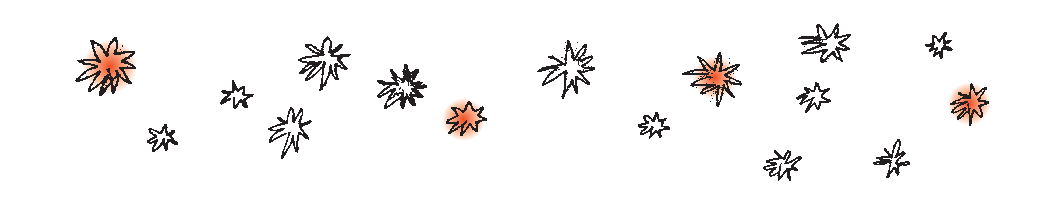
\includegraphics{art/202502_kol16}}\vskip-10pt
\normalsize

\def\zadMat#1{%
  \textbf{M~#1.} \csuse{zadM-#1}%\\%
  %Rozwiązanie na str.~\pageref{rozM-#1}%
}
\def\zadFiz#1{%
  \textbf{F~#1.} \csuse{zadF-#1}%\\%
 % Rozwiązanie na str.~\pageref{rozF-#1}%
}

\renewcommand{\Zadania}[1][0pt]{%
\zadspis
\phantomsection\label{zadania}\noindent\setbox0=\hbox to70pt{
\includegraphics{kot}\hss}%
\copy0{\Magenta{\LARGE\bf Zadania}}}
\marg[-2]{\Zadania\vskip20pt
}%
\redaguje{Przygotował  Dominik BUREK}

\zadMat{1807}

\zadMat{1808}

\zadMat{1809}

\redaguje{Przygotował Andrzej MAJHOFER}

\zadFiz{1113}



\marg[69]{\normalsize
\Magenta{\bf Rozwiązania na str.~\pageref{rozwiazania}}}\zadFiz{1114}

\eject